\documentclass[aps, pra, 10pt, twocolumn, superscriptaddress,floatfix]{revtex4-1}

\usepackage{amsmath,amssymb,amsfonts}
\usepackage{braket}
\usepackage[breaklinks=true,colorlinks,citecolor=blue,linkcolor=blue,urlcolor=blue]{hyperref}
\usepackage{mathtools}
\usepackage{dsfont}
\usepackage{algorithm}
\usepackage{algc}
\usepackage{algcompatible}
\usepackage{algpseudocode}
%

%%
\def \id {\mathds{1}}
\def \abs {\text{Abs}}
\newcommand{\norm}[1]{\lVert#1\rVert}
\DeclareMathOperator{\tr}{Tr}
\newcommand{\round}[1]{\ensuremath{\lfloor#1\rceil}}
\newcommand{\mi}{\mathrm{i}} %% roman "i"
%

\begin{abstract}
	In this notes we comment on the possibility of applying the Granade Bayesian phase estimation algorithm to our q-plate experiment. The first thing that we can do is to verify that the Bayesian approach reproduces the results of our non-adaptive procedure.
\end{abstract} 
%

\begin{document}
%
\title{Notes on the Bayesian phase estimation} 
%


\author{Federico Belliardo}
\email{federico.belliardo@sns.it}
\affiliation{NEST, Scuola Normale Superiore, I-56126 Pisa,~Italy}

\maketitle

\section{Bayesian algorithm}
%
In this note we apply the Bayesian algorithm presented by Granade~\cite{Granade2012} to our q-plates setup, with a few corrections due to the circular nature of the angular variable that we are going to measure. In every simulated experiment  a constant number of particles equal to $n_p = 1000$ or $n_p = 5000$ has been used. The parameters to estimate are collected in the vector $\boldsymbol{x} := \left( \theta, V_1, V_2, V_3, V_4 \right)$, that contains the phase in the first entry and the four visibilities in the other ones. Being the Granade's method based on a particle filter, it represents internally the posterior probability distribution with the ensemble $\mathcal{E} := \lbrace \boldsymbol{x}^i, w^i \rbrace$, where $\boldsymbol{x}^i$ is the position of the $i$-th particle and $w^i$ its weight. The $j$-th component of the $i$-th particle of the ensemble will be represented as $x_j^i$, and could correspond to the phase if $j=0$, that is $x^i_0 = \theta^i$ or to one of the visibilities if $j=1, 2, 3, 4$, that is $x^i_j = V^i_j$. The mean of the angular values is computed as
%
\begin{equation}
	\hat{\mu}_0 := \arg \left[ \sum_{i=1}^{n_{p}} w^i \exp \left( \mi \theta^i \right) \right] \; ,
\end{equation}
%
while the mean values of the visibilities are
%
\begin{equation}
	\hat{\mu}_j = \sum_{i=1}^{n_p} w^i V^i_j \; .
\end{equation}
%
Together they form the vectorial mean of the distribution $\boldsymbol{\hat{\mu}} = (\hat{\mu}_0, \hat{\mu}_1, \hat{\mu}_2, \hat{\mu}_3, \hat{\mu}_4)$. The covariance matrix is defined as
%
\begin{equation}
	\text{Cov}_{ij} := \sum_{k=1}^{n_{p}} w^k (x^k_i - \hat{\mu}_i)  (x^k_j - \hat{\mu}_j) \; .
\end{equation}
%
If $i=1$ or $j=1$ then difference in $x^k_i - \hat{\mu}_i$ or $x^k_j - \hat{\mu}_j$ is actually the circular distance
%
\begin{equation}
	d(x^k_i, \hat{\mu}_i) = \pi - | (x^k_i - \hat{\mu}_i) \mod 2 \pi - \pi| \; .
\end{equation}
%
In the utility function we have considered only the variance of the phase, that is the component $\text{Cov}_{11}$ of the covariance matrix, so that the visibilities are treated as \textbf{nuisance parameters}. The resampling strategy of the Granade procedure has also undergone minor changes to adapt it to the phase estimation problem. We have simulated both algorithms (we didn't use the actual experimental data collected) with visibilities $V_1 = 0.90$, $V_2 = 0.875$, $V_3 = 0.850$ and $V_4 = 0.765$. The error of the iterative algorithm is the mean error of $100$ equally spaced angles in $[0, 2 \pi)$, while all the Bayesian experiments are estimations of the particular angle $\theta = 2$. In Fig.~\ref{fig:30000.pdf} we report the simulation performed for up to $N = 30000$ resources, done with $n_p = 1000$.
%
\begin{figure}[!t]
	\begin{center}
		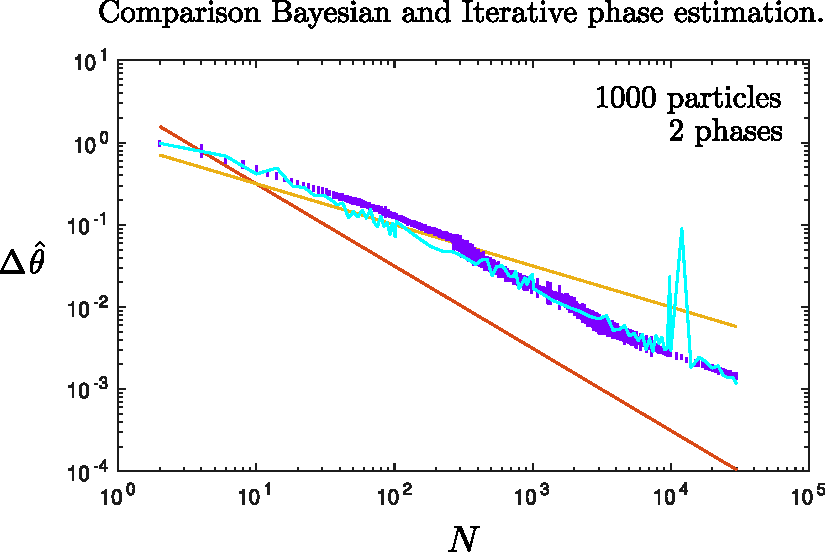
\includegraphics[width=0.5\textwidth]{immagini/30000.pdf}
	\end{center}
	\caption{The light blue line is the RMSE of the Bayesian simulation (plot without the error bars), while the violet plot is the RMSE achieved via the iterative phase estimation algorithm (with error bars). The yellow and red lines are respectively the standard quantum limit ($\Delta \hat{\theta} = 1/\sqrt{N}$) and the Heisenberg scaling ($\Delta \hat{\theta} = \pi/N$). The Bayesian approach beats the iterative one for low resource numbers $N \sim \mathcal{O} (100)$. It has to be observed that near $N \sim 10^4$ the Bayesian procedure fails. In the simulations of the iterative phase estimation $100$ experiments have been performed for each particle number, while in the Bayesian one only $30$. In both estimation algorithms we were allowed only to use two types of polarization measurements on the photons, i.e. the Type-$0$ and Type-$+$ measurements used in~\cite{Belliardo2020}.}
	\label{fig:30000.pdf}
\end{figure}
%
The simulation has ben repeated in the same conditions also for $n_p = 5000$, and the results are given in Fig.~\ref{fig:30000part5000.pdf}.
%
\begin{figure}[!t]
	\begin{center}
		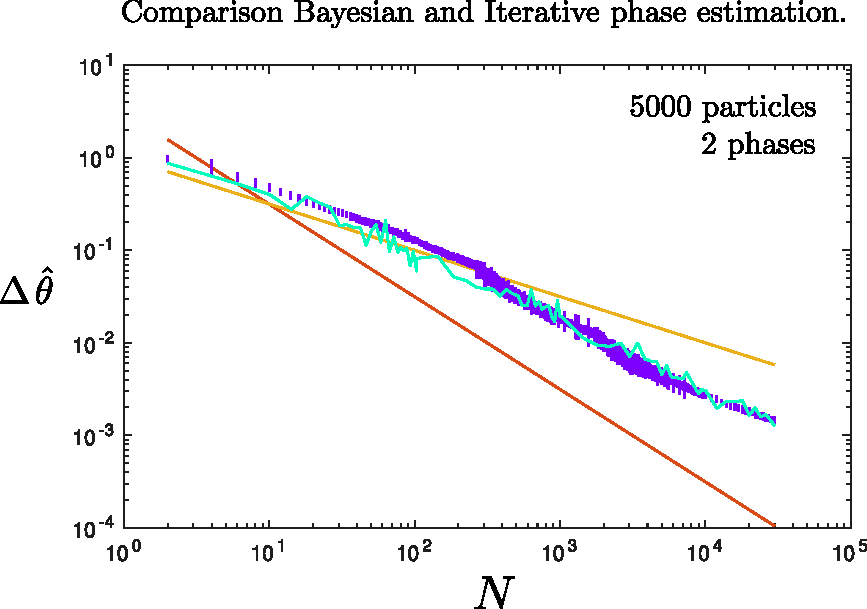
\includegraphics[width=0.5\textwidth]{immagini/30000part5000.pdf}
	\end{center}
	\caption{This plot contains the results of a simulation performed with the same conditions of Fig.~\ref{fig:30000.pdf}, but with $n_p = 5000$ for the particle filter. The light blue line is the RMSE of the Bayesian simulation (plot without the error bars), while the violet plot is the RMSE achieved via the iterative phase estimation algorithm (with error bars). The yellow and red lines are respectively the standard quantum limit ($\Delta \hat{\theta} = 1/\sqrt{N}$) and the Heisenberg scaling ($\Delta \hat{\theta} = \pi/N$).}
	\label{fig:30000part5000.pdf}
\end{figure}
%
We might try to expand the number of possible polarization measurements on the photons, and again select the optimal one each times. A simulation with $32$ different possible measurements, with corresponding angles equally spaced in $[0, 2 \pi)$, has been performed, and the results are reported in Fig.~\ref{fig:5800.pdf}.
%
\begin{figure}[!t]
	\begin{center}
		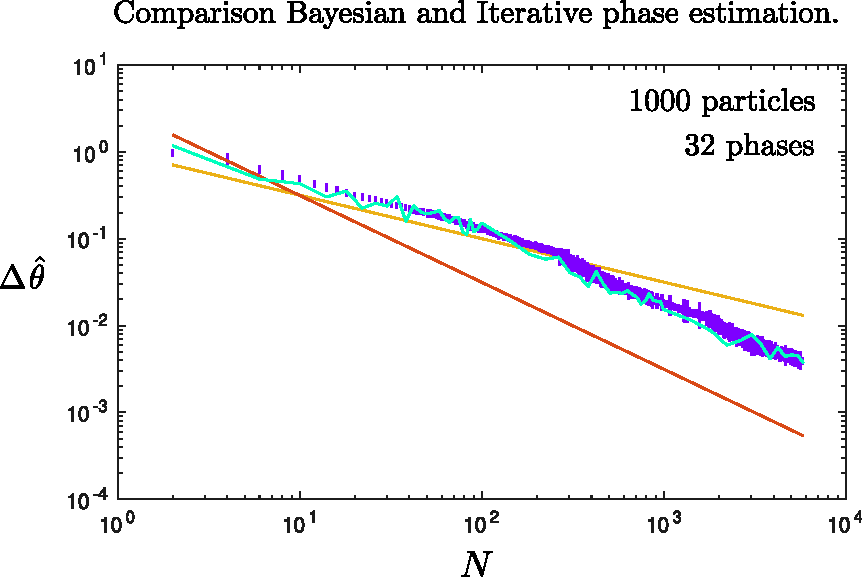
\includegraphics[width=0.5\textwidth]{immagini/5800.pdf}
	\end{center}
	\caption{The light blue line is the RMSE of the Bayesian simulation (plot without the error bars), while the violet plot is the RMSE achieved via the iterative phase estimation algorithm (with error bars). The yellow and red lines are respectively the standard quantum limit ($\Delta \hat{\theta} = 1/\sqrt{N}$) and the Heisenberg scaling ($\Delta \hat{\theta} = \pi/N$). The simulation has been performed wit $32$ possible polarization measurements on the codified photons, and with $n_p = 1000$ particles. The violet lines still refer to the same simulation performed with two only two polarization measurements.}
	\label{fig:5800.pdf}
\end{figure}
%
The failure of the Bayesian procedure that is observed in Fig.~\ref{fig:30000.pdf} is not observed in Fig.~\ref{fig:30000part5000.pdf}. The Bayesian procedure can't formally guarantee that the error will be under a certain threshold and we cannot claim with certainty that the failure of the Bayesian estimation is caused by the low number of particles used in the filter and that it will be solved by increasing this number. In Fig.~\ref{fig:5800.pdf} it strangely seems that the consistent advantage that the Bayesian procedure showed for $N \sim \mathcal{O} (100)$ is lost. Using $32$ measurements gives precisions which are in accordance with the lower end of the error bars of the iterative procedure. We underline that the precisions of the Bayesian experiments that we have done seem to be much more fluctuating than the precision we get from the iterative procedure, but it may be due to the small statistics (only $30$ experiments for each point) and to the use of only one angle $\theta = 2$.
%

\section{Comment on the case of fluctuating visibilities}
\label{sec:fluctVisibilities}
%
In this section we briefly analyse what happens if the visibilities are also fluctuating quantities. This observations apply also to the iterative phase estimation procedure of~\cite{Cimini2021}. Suppose that the visibility of a q-plate is a stochastic variable $V$ extracted from a distribution $\mathcal{P} (V)$. Then the outcome probability of a polarization measurement on a photon is
%
\begin{equation}
	p_0 = \int dV p_0^V \mathcal{P} (V) \; ,
	\label{eq:defip0}
\end{equation}
%
where 
%
\begin{equation}
	p_0^V = \frac{1+V \cos(s \theta)}{2} \; .
	\label{eq:prob}
\end{equation}
%
Substituting Eq.~\eqref{eq:prob} in Eq.~\eqref{eq:defip0} we get
%
\begin{equation}
	p_0 = \int dV \frac{1+V \cos(s \theta)}{2} \mathcal{P} (V) \;  = \frac{1 + \mu_V \cos(s \theta)}{2} \; .
	\label{eq:der}
\end{equation}
%
where $\mu_V$ is the mean visibility. Therefore if the visibilities are fluctuating variables, only the their mean value is necessary to compute the resource distribution~\cite{Cimini2021}. Similarly in a Bayesian approach we only need to learn the mean visibilities, that are encoded in the outcome distribution in Eq.~\eqref{eq:der} with the same form of regular visibilities. When performing an estimation with known (unknown) visibilities $V_1, V_2, V_3, V_4$ we can indifferently say that these are (we are learning) the actual visibilities or that these are (we are learning) the mean values of the visibility distributions. 

\section{Idea of the paper}
%
After a discussion with Valeria, Emanuele, and Francesco we have decided to write a paper which will show in the experimental context of photonics a quantum advantage for multiparameter estimation with nuisance parameter. That is, we want to write a paper which could be considered as the follow up of both~\cite{Cimini2021} and~\cite{Roccia2018}. We want to approach a problem of multiparameter quantum quantum estimation with limited unknown visibilities and add also the possibility of having quantum enhanced precision. 

We can assume the visibilities $V_i$ of the $i$-th q-plate to be extracted from the distributions $\mathcal{P}_i(V_i)$. We will try the following two algorithms
%
\begin{itemize}
	\item the iterative phase estimation algorithm with photon distributions computed using as visibilities the mean values $\mu_V^i$ of each distributions $\mathcal{P}_i(V_i)$. This algorithm uses at best the prior information we have on the visibilities, but computes the photon distribution offline, and doesn't try to learn it on the fly.
	
	\item the Bayesian phase estimation of Granade~\cite{Granade2012}, which will start from the priors $\mathcal{P}_i(V_i)$ and gradually learn the actual visibilities $V_i$.
\end{itemize}
%
Both algorithms, our offline estimation and the online algorithm of Granade, are working at the best of their possibilities. The iterative algorithm \textbf{can} take into account fluctuating visibilities, but only by incorporating a certain prior and not by learning like the Bayesian counterpart. Considering only the prior is the best we can do if we must produce a strategy (the photon distribution) before a measurement is even done.

We can choose $P_i (V_i)$ among three possibilities: a uniform distribution in $[0, 1]$, a uniform distribution in $[0.5, 1]$, or a Gaussian distribution. The real $V_i$ are the experimental one, that is $V_1 = 0.90$, $V_2 = 0.875$, $V_3 = 0.850$ and $V_4 = 0.765$, but if the prior are uniform then the best the offline algorithm can do is use as visibilities $\mu_V^i = 0.5$, for example. We have the measured data for the actual experimental visibilities (from the experiment in~\cite{Cimini2021}) and we compare how the two algorithms  work when they are initially only given a prior. We should expect to see the iterative algoruthm lag behind the Bayesian one. 

With this experiment we are exploring the regime of quantum enhanced estimation with nuisance parameters in the naturally multiparametric context of optical experiments.

\section{Some technical notes}
%
In this section I add some technical notes.
%
\begin{itemize}
	\item Performing the Bayesian analysis for $200$ repetitions of the same experiment and for $20$ phases will take too long. We should concentrate on a single phase or considerably reduce the number of repetition of the each single experiment.
	
	\item The way the Bayesian procedure is adapted to be performed for a fixed number of total resources introduces an imprecision on the $x$ values ($N$) of the plots in Fig.~\ref{fig:30000.pdf},~\ref{fig:30000part5000.pdf}, and~\ref{fig:5800.pdf}. Therefore we will need to add not only a vertical error bar, but also an horizontal one.
	
	\item It might be interesting to find which visibility affects the most the error. For this purpose we might try to estimate jointly the phase and one of the visibility $V_i$, which won't be treated as a nuisance parameter.
	
\end{itemize}

\begin{thebibliography}{100}
	
	\bibitem{Granade2012} C E Granade \textit{et al.} 2012 \href{https://doi.org/10.1088/1367-2630/14/10/103013}{New J. Phys. {\bf 14} 103013}.
	%
	
	\bibitem{Cimini2021} V Cimini \textit{et al.}, \href{http://arxiv.org/abs/2110.02908}{arXiv:2110.02908 (2021).}
	
	\bibitem{Belliardo2020} F Belliardo and V Giovannetti, \href{https://link.aps.org/doi/10.1103/PhysRevA.102.042613}{Phys. Rev. A~{\bf 102}, 042613}.
	
	\bibitem{Roccia2018} E Roccia \textit{et al.}, \href{https://www.osapublishing.org/optica/abstract.cfm?uri=optica-5-10-1171}{Optica~{\bf 5}, 1171-1176 (2018).}
	
\end{thebibliography}

\end{document}